In this chapter we use the paper "Do LoRa Low-Power Wide-Area Networks Scale?" by M. Bor et al. and the LoRa simulator LoRaSim to reproduce the figures reporting the results of two Experiments Sets from the paper. LoRaSim is a simulator based on SimPy for simulating collisions in LoRa networks and consists in four Python scripts simulating different types of network, that can be run setting some parameters. In order to replicate the two figures, we need to understand which transmitter configuration was user for every configuration SN\textsuperscript{i} and use the correct simulator with the correct parameters.

\section{Figure 5: Experiment Set 2}
The Experiment Set 2 evaluates the impact of dynamic communication parameter selection on the Data Extraction Rate (DER) and compares three transmitter configurations, called  SN\textsuperscript{3}, SN\textsuperscript{4} and SN\textsuperscript{5} in the paper.\\
First of all, we need to choose the correct Python script in the simulator; the paper says that nodes transmit to a single sink (M=1), so we choose the script loraDir.py. From the LoRaSim documentation, we check the parameters used from the selected script, that are reported here:
\begin{BreakableVerbatim}
./loraDir.py <NODES> <AVGSEND> <EXPERIMENT> <SIMTIME> [COLLISION]
\end{BreakableVerbatim}
For all experiments, we choose:
\begin{itemize}
\item The number of nodes, <NODES>, is chosen from a list built based on the data point of Figure 5 from the paper.
\item The average sending interval in milliseconds, <AVGSEND>, is set to 1 million of milliseconds, i.e. 16.7 minutes.
\item The simulation time, <SIMTIME>, is not specified from the paper; we choose a simulation time of 58 days, the same as the one used in Experiment Set 1.
\item We set <COLLISION> to 1 to enable the full collision check.
\end{itemize}
The key difference between the different configurations is represented by the <EXPERIMENT> parameter that determines with which radio settings the simulation is run. We are going to choose the experiment looking at how the Experiment Set is described and at the LoRaSim documentation. The paper says that SN\textsuperscript{3} uses the settings used by common LoRaWAN deployments, which refers to <EXPERIMENT> = 4. SN\textsuperscript{4}, instead, is the configuration that minimizes the airtime for each node, by setting the BW, SF and CR, with constant TP; this description corresponds to <EXPERIMENT> = 3. Finally, SN\textsuperscript{5} minimizes first airtime and then Transmission Power, as done by the simulator with <EXPERIMENT> = 5.

The complete code used to simulate the network with LoRaSim and plot the DER is reported here.
\begin{python}
import os
import subprocess
import math
import pandas as pd
import matplotlib
import matplotlib.pyplot as plt

def simulate(n_nodes, tx_rate, exp, duration):
    env = os.environ.copy()
    env["MPLBACKEND"] = "Agg"
    # Use subprocess.run to execute the command and capture output
    result = subprocess.run(
        [
            "python2",
            "lorasim/loraDir.py",
            str(int(n_nodes)),
            str(int(tx_rate)),
            str(int(exp)),
            str(int(duration)),
            str(int(1))
        ],
        env=env,
        capture_output=True,
        text=True,  # Capture output as text
    )

# Der in aloha defined as S/G = e^(-2G)
def aloha_der(n_nodes,t):
    rate = 1e-6
    return math.exp(-2 * n_nodes * rate * t)

def main():
    duration = 58 * 86400000
    tx_rate = 1e6

    for n_nodes in list(range(1,10)) + list(range(10,100,10)) + list(range(100,1000,100)) + list(range(1000,1601,200)):
        print(f"Simulating {n_nodes} nodes")
        simulate(n_nodes, tx_rate, 4, duration)
        simulate(n_nodes, tx_rate, 3, duration)
        simulate(n_nodes, tx_rate, 5, duration)

    data_sn3 = pd.read_csv("exp4.dat", sep=" ")
    data_sn4 = pd.read_csv("exp3.dat", sep=" ")
    data_sn5 = pd.read_csv("exp5.dat", sep=" ")
    data_sn3["der"] = (data_sn3["nrTransmissions"] - data_sn3["nrCollisions"]) / data_sn3["nrTransmissions"]
    data_sn4["der"] = (data_sn4["nrTransmissions"] - data_sn4["nrCollisions"]) / data_sn4["nrTransmissions"]
    data_sn5["der"] = (data_sn5["nrTransmissions"] - data_sn5["nrCollisions"]) / data_sn5["nrTransmissions"]
    
    plt.plot(data_sn3["#nrNodes"], data_sn3["der"], marker = 'o', label="SN3")
    plt.plot(data_sn4["#nrNodes"], data_sn4["der"], marker = 'o', label="SN4")
    plt.plot(data_sn5["#nrNodes"], data_sn5["der"], marker = 'o', label="SN5")
    plt.title("Success Rate (%)")
    plt.xlabel("Number of nodes")
    plt.ylabel("Rate")
    plt.legend()
    plt.grid()

    plt.savefig("figure5.pdf")
    plt.show()

if __name__ == '__main__':
    main()
\end{python}

The plot that corresponds to Figure 5 from the paper is reported here.

\begin{figure}[H]
    \centering
    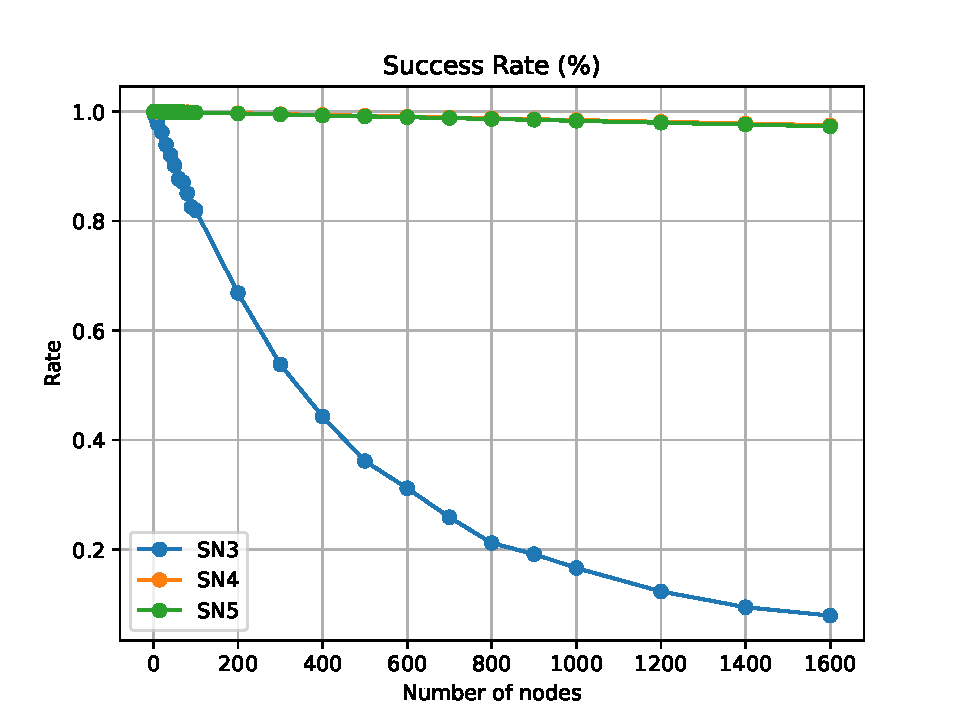
\includegraphics[width=0.7\linewidth, height=0.5\textheight, keepaspectratio]{figure5_58d_collision.pdf}
    \caption{Plot corresponding to Figure 5: Experiment Set 2}
\end{figure}

\section{Figure 7: Experiment Set 3}
The Experiment Set 3 analyzes the impact of the number of sinks M on the network performance, while Figure 7 focuses on the impact on the DER. The experiment uses the configuration called SN\textsuperscript{1}, with SF = 12, BW = 125 kHz and CR = 4/8, and tests different numbers of sinks (1, 2, 3, 4, 8, 24).\\
The Python script of the LoRaSim simulator that allows to test multiple sinks is loraDirMulBs.py and takes the following parameters:
\begin{BreakableVerbatim}
./loraDirMulBS.py <NODES> <AVGSEND> <EXPERIMENT> <SIMTIME> <BASESTATIONS> [COLLISION]
\end{BreakableVerbatim}
The only new parameter with respect to the previous Experiment Set is <BASESTATIONS> which is the number of gateways we have in the network. 
The parameters that are common to Experiment Set 2 are: 
\begin{itemize}
\item Parameter <NODES>, chosen from the same list of numbers.
\item <AVGSEND> is set to 1 million of milliseconds.
\item <COLLISION> is set to 1.
\end{itemize}
We modified the <SIMTIME> to 1 day, because it is not specified by the paper and Google Colab can't handle a very long simulation time for this Experiment Set, since it saturates the available RAM. The paper says that the used setting is the one of SN\textsuperscript{1}, which uses the most robust LoRa transmitter settings leading to transmissions with the longest possible airtime and with fixed Carrier Frequency. This description refers to <EXPERIMENT> = 0, which uses a constant frequency. The number of gateways, contained in the parameter <BASESTATIONS> changes among the different simulations and is set to 1, 2, 3, 4, 8 and 24, as done in the paper.
The complete code used to simulate the network with LoRaSim and plot the DER is reported here.

\begin{python}
import os
import subprocess
import math
import pandas as pd
import matplotlib
import matplotlib.pyplot as plt

def simulate(n_nodes, tx_rate, exp, duration):
    env = os.environ.copy()
    env["MPLBACKEND"] = "Agg"

    # Use subprocess.run to execute the command and capture output
    result = subprocess.run(
        [
            "python2",
            "lorasim/loraDir.py",
            str(int(n_nodes)),
            str(int(tx_rate)),
            str(int(exp)),
            str(int(duration)),
            str(int(1))
        ],
        env=env,
        capture_output=True,
        text=True,  # Capture output as text
    )

# Der in aloha defined as S/G = e^(-2G)
def aloha_der(n_nodes,t):
    rate = 1e-6
    return math.exp(-2 * n_nodes * rate * t)

def main():
    duration = 30 * 86400000
    tx_rate = 1e6

    for n_nodes in list(range(1,10)) + list(range(10,100,10)) + list(range(100,1000,100)) + list(range(1000,1601,200)):
        print(f"Simulating {n_nodes} nodes")
        simulate(n_nodes, tx_rate, 0, duration, 1)
        simulate(n_nodes, tx_rate, 0, duration, 2)
        simulate(n_nodes, tx_rate, 0, duration, 3)
        simulate(n_nodes, tx_rate, 0, duration, 4)
        simulate(n_nodes, tx_rate, 0, duration, 8)
        simulate(n_nodes, tx_rate, 0, duration, 24)

    data_bs_1 = pd.read_csv("exp0BS1.dat", delim_whitespace=True, comment="#", names=["nrNodes", "DER"])
    data_bs_2 = pd.read_csv("exp0BS2.dat", delim_whitespace=True, comment="#", names=["nrNodes", "DER"])
    data_bs_3 = pd.read_csv("exp0BS3.dat",delim_whitespace=True, comment="#", names=["nrNodes", "DER"])
    data_bs_4 = pd.read_csv("exp0BS4.dat", delim_whitespace=True, comment="#", names=["nrNodes", "DER"])
    data_bs_8 = pd.read_csv("exp0BS8.dat", delim_whitespace=True, comment="#", names=["nrNodes", "DER"])
    data_bs_24 = pd.read_csv("exp0BS24.dat", delim_whitespace=True, comment="#", names=["nrNodes", "DER"])
   
    plt.plot(data_bs_1["nrNodes"], data_bs_1["DER"], marker = 'o', label="1 sink")
    plt.plot(data_bs_2["nrNodes"], data_bs_2["DER"], marker = 'o', label="2 sink")
    plt.plot(data_bs_3["nrNodes"], data_bs_3["DER"], marker = 'o', label="3 sink")
    plt.plot(data_bs_4["nrNodes"], data_bs_4["DER"], marker = 'o', label="4 sink")
    plt.plot(data_bs_8["nrNodes"], data_bs_8["DER"], marker = 'o', label="8 sink")
    plt.plot(data_bs_24["nrNodes"], data_bs_24["DER"], marker = 'o', label="24 sink")
    plt.title("Success Rate (%)")
    plt.xlabel("Number of nodes")
    plt.ylabel("Rate")
    plt.legend()
    plt.grid()
    plt.savefig("figure7.pdf")
    plt.show()

if __name__ == '__main__':
    main()

\end{python}

The plot that corresponds to Figure 7 from the paper is reported here.
\begin{figure}[H]
    \centering
    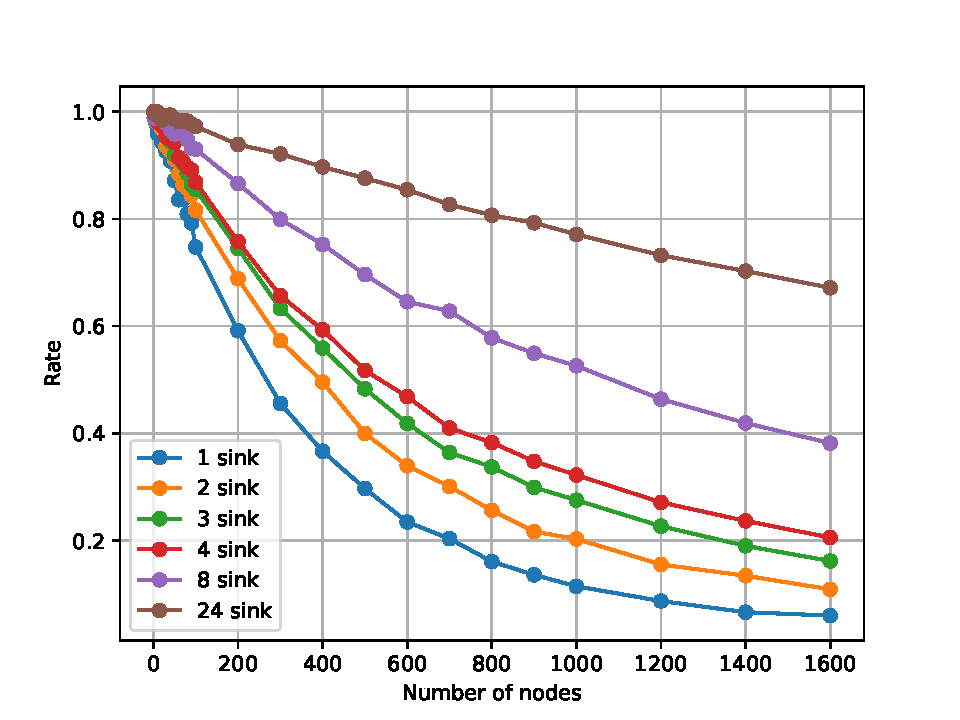
\includegraphics[width=0.7\linewidth, height=0.5\textheight, keepaspectratio]{figure7_exp0_1d_collision.pdf}
    \caption{Plot corresponding to Figure 7: Experiment Set 3}
\end{figure}


